\documentclass[a4paper,11pt]{amsart}
\usepackage{amssymb}
\usepackage[T1]{fontenc}
\usepackage{indentfirst}
\usepackage{enumerate}
\usepackage{stmaryrd}
\usepackage{xspace}
\usepackage{amsmath}
\usepackage{amsfonts}
\usepackage{url}
\usepackage[colorlinks=true, a4paper=true, pdfstartview=FitV,
linkcolor=blue, citecolor=blue, urlcolor=blue]{hyperref}
\pdfcompresslevel=9

\usepackage[left=2.61cm,right=2.61cm,top=2.72cm,bottom=2.72cm]{geometry}


\usepackage{graphicx}
%%%%%%%for quotes
\usepackage{textcmds}

\usepackage[english,frenchb]{babel}
%\usepackage[latin1]{inputenc}
\usepackage[utf8]{inputenc}
\usepackage{indentfirst, amsfonts, amsmath, amsthm, amssymb, amscd}
\usepackage{amsmath,amsfonts,amscd,bezier}
%%%%%%%%%%%%%%%%%%%%%%%%%
\usepackage[most]{tcolorbox}
%%%%%symbol for EUR
\usepackage{eurosym}
%%%%%%%%
\begin{document}
\begin{tcolorbox}[center,colback=white]
\begin{center}
{\large\textsc{Estimate Compressive Strength of Concrete}}\\
\end{center}
\end{tcolorbox}

\section{Description}

In this project, we employ regression methods to predict the concrete compressive strength in terms of MPa (megapascal). Concrete is one of the most important material in civil engineering since it is used for the development of foundations, columns, beams, slabs, and different load-bearing components. The concrete compressive strength is a highly nonlinear function of age and ingredients. The actual concrete compressive strength (MPa) for a given mixture under a specific age (days) was determined from a laboratory. Our goal is to predict the concrete compressive strength. To do that, we analyse the different regression methods (Multilinear, Ridge, Lasso, and Elastic Net), and we can compare their error metrics and their scores. As an optional analysis, we employ statsmodels and compare all the results. 

\medbreak 

The data set used in this project is available on the Machine Learning Repository of University of California, Irvine \href{https://archive.ics.uci.edu/ml/datasets/Concrete+Compressive+Strength}{Concrete Compressive Strength Data Set (UC Irvine)}. The UCI page mentions the following publication as the original source of the data set:

\medbreak

\begin{flushleft}
1 - Cheng Yeh,\emph{"Modeling of strength of high performance concrete using artificial neural networks,"} Cement and Concrete Research, Vol. 28, No. 12, pp. 1797-1808 (1998).
\end{flushleft}

\medbreak

Now, let us briefly explain how we plan to present our analysis and result. In the first stage, we get the data, prepare/clean it, and define features. Then we make some plots, so we can visualize the outliers of the response/target variable. To get a flavour of the techniques used in this project we make a simple linear regression. More precisely, we pick one feature (\texttt{`Cement (kg/$m^3$)'}) and quantify its relationship with the target (\texttt{`Concrete Compressive Strength (MPa)'}), see Section \ref{dataanalysis} below for more details. then, we dive into the regularization techniques, where we give details of the tools used in Multilinear, Ridge, Lasso, and Elastic Net methods. As a bonus, we also employ statsmodels library to obtain R-squared and MSE values.

\medbreak

In Section \ref{problem}, we present the formal problem and mention our target audience. In Section \ref{dataanalysis}, we explain the data cleaning, data visualization, and regression methods. In Section \ref{results}, we present the key findings of our analysis and discuss the results obtained in this project. Finally, in Section {future}, we discuss about the accuracy of each method, and possible ways to improve them.

\medbreak

Finally, we mention that in order to clarify our analysis, and give a clean presentation of the results therein obtained, we add the notebook file to this report. In this way, the reader can easily follow the graphes and ideas described in this project.

\section{Problem Statement \& Target Audience}\label{problem} 

Our goal is to predict the concrete compressive strength by using regression methods. Most engineering construction uses cement concrete composites as the main building material. Needless to say, the concrete plays a very important role in all branches of civil engineering. An important fact is that concrete can be manufactured to the desired strength with an economy. In other words, construction workers can optimize the strength by knowing the exact ratio of the components that make the concrete. However, compared to other binding materials, the tensile strength of concrete is relatively low. Therefore, it is important for companies to increase their levels of strength of concrete.
Finally, our target is any company in the branch of civil engineering.

\section{Data Analysis}\label{dataanalysis}

We begin our analysis by getting the data set, which is available on the Machine Learning Repository of University of California, Irvine \href{https://archive.ics.uci.edu/ml/datasets/Concrete+Compressive+Strength}{Concrete Compressive Strength Data Set (UC Irvine)}. This dataset contains data on the components of a concrete, and the concrete compressive strength MPa. Here are some basic information,

\medbreak

\begin{flushleft}
Number of instances: $1030$\\
Number of Attributes: $9$\\
Attribute breakdown $8$ quantitative input variables, and $1$ quantitative output variable\\
Missing Attribute Values None
\end{flushleft}

\medbreak

The features (input variables), which are all of quantitative type, are given by
\begin{flushleft}
\texttt{`Cement (component 1) --  kg in a $m^3$ mixture'}\\
\texttt{`Blast Furnace Slag (component 2) --  kg in a $m^3$ mixture'}\\
\texttt{`Fly Ash (component 3) --  kg in a $m^3$ mixture'}\\
\texttt{`Water (component 4) --  kg in a $m^3$ mixture'}\\
\texttt{`Superplasticizer (component 5) --  kg in a $m^3$ mixture'}\\
\texttt{`Coarse Aggregate (component 6) -- kg in a $m^3$ mixture'}\\
\texttt{`Fine Aggregate (component 7) --  kg in a $m^3$ mixture'}\\
\texttt{`Age -- Day (1~ 365)'}
\end{flushleft}
and the target/response (output variable), which is also of quantitative type, is given by
\begin{flushleft}
\texttt{`Concrete compressive strength -- MPa'}
\end{flushleft}

\medbreak

Once we identify the types of our features we proceed to our next stage: Data Cleaning. Therein, we check for missing values, change headers of columns, and create the feature matrix $X$, and the response vector $y$. Next, we use box-plot to visualize the target/response, so we can identify the outliers. Then, we employ the interquartile range (IQR) to remove the outliers. there are other ways to remove the outliers, e.g., the z-score, but we only use the IQR in this project. After dropping the outliers, the feature matrix reduces to $941$ rows and $8$ columns. 

\medbreak

As a straightforward exercise, we make a simple linear regression, where we take into account only the feature \texttt{`cement'}. This gives us a flavour of the regression methods, which are the central part of this project. 

\medbreak

Then, with the help of scikit-learn library, we dive into the regression methods: Multilinear, Ridge, Lasso, and Elastic Net.

\medbreak

\noindent{\textsc{Multilinear}:} We first observe that by adding more variables to the model, it increases the average \texttt{`neg mean squared error'} from almost $-296.35$ to about $-70.37$, which is a considerable improvement. In order words, more variables imply in a lower error metric. Then, we discuss the values of the coefficients, which are obtained with or without scaling. At that point, we should take into account that it is important to scale the data, which we do by using StandarScaler, before performing Ridge Regression. The reason is that Ridge is sensitive to the scale of the input features. Then, we plot a graph of the coefficients and observe that the features \texttt{`Water ($kg/m^3$)'}, \texttt{`Superplasticizer ($kg/m^3$)'}, and \texttt{`Age (day)'} have a considerable impact on \texttt{`Concrete Compressive Strength (MPa)'}.

\medbreak

\noindent{\textsc{Regularization: Ridge, Lasso, and Elastic Net.}} We first explore the correlation matrix of $X$, so we can study the correlation between the features, and establish their importance for predicting our target. We visualize the correlation analysis with heatmap, which is handy to better identify the features and their correlations. Then, we import the functions Ridge, Lasso, and ElasticNet from \texttt{sklearn linear models}, and obtain the scores, MSE, and coefficients, which we discuss in more details in Section \ref{results}. 

\medbreak

\noindent{\textsc{GridSearchCV Algorithm}:} Our result show that these three models give very similar results. So, we will split the data into training and test sets, build Ridge, Lasso, and Elastic Net, and choose the regularization parameter with the help of GridSearch. For that, we have to define the set of parameters for GridSearch. In this case, the models with the highest R-squared score will give us the best parameters.

\medbreak

\noindent{\textsc{Statsmodels}:} As a bonus, in the final part of this project we employ statsmodels  for our linear regression. This library has convenient ways to specify parameters. 

\section{Key Findings}\label{results}

Let us begin with an analysis of the multilinear method. When we take into account only the feature \texttt{`cement (kg in $m^3$)'} to predict the response, we obtain
$$
-296.35,
$$ 
as the mean of MSE, which is used as an indicator of how good the model is. Then, by adding all the other features, we obtain 
$$
-70.37,
$$
which implies in a considerable improvement. In regard with regularization, we know that it is crucial to scale the data. So, we obtain the following table for the coefficients 
\begin{table}[h!]
  \begin{center}
    \caption{\textsc{Coefficients}}
    \label{tab:table1}
    \begin{tabular}{l|c|r} 
      & \textbf{Without Scaling} & \textbf{Scaled}\\
      \hline
      \text{Cement($kg/m^3$)} &0.102002&	10.387271\\
      \text{Blast Furnace Slag($kg/m^3$)} & 0.075504 &6.516875\\
      \text{Fly Ash($kg/m^3$)} & 0.048206 &3.101027\\
      \text{Water($kg/m^3$)} &-0.249595 & -4.677350\\
      \text{Superplasticizer($kg/m^3$)} &0.216019 &1.153038\\
      \text{Coarse Aggregate($kg/m^3$)} &-0.010251&-0.795538\\
      \text{Fine Aggregate($kg/m^3$)}&-0.010303& -0.773074\\
      \text{Age(Day)}&0.312695&	8.925410\\
    \end{tabular}
  \end{center}
\end{table}

Using matplotlib we observe that the features Water ($kg/m^3$), Superplasticizer ($kg/m^3$), and Age (day) have a considerable impact on Concrete Compressive Strength (MPa).

\medbreak

Now, let us describe our results obtained in the regularization part. 

\medbreak

\noindent{\textsc{Ridge:}}
\begin{flushleft}
The value of the Ridge Score is:  $0.7699$\\
The value of the Ridge MSE is:  $63.25$\\
The value of the Ridge coefficients are given by:  $(10.387,  6.516,  3.101, -4.677,  1.153, -0.795,
  -0.773,  8.925)$
\end{flushleft}

\medbreak

\noindent{\textsc{Lasso:}}
\begin{flushleft}

The value of the LASSO Score is:  $0.7699$\\
The value of the LASSO MSE is:  $63.25$\\
The value of the LASSO coefficients are given by:  $(10.386,  6.516,  3.100, -4.677,   1.153,  -0.795,
 -0.773,  8.925)$
\end{flushleft}

\medbreak

\noindent{\textsc{Elastic Net}:}
\begin{flushleft}
The value of the Elastic Net Score is:  $0.7699$\\
The value of the Elastic Net MSE is:  $63.25$\\
The value of the Elastic Net coefficients are given by: $(10.381,  6.511,   3.095, -4.680,  1.153, -0.799,
 -0.777,  8.924)$
\end{flushleft}

\medbreak

Our analysis shows that these three models give very similar results. So, we split the data into training and test sets, build Ridge, Lasso, and Elastic Net, and choose the regularization parameter with the help of GridSearch. For that, we have to define the set of parameters for GridSearch. In this case, the models with the highest R-squared score will give us the best parameters. We refer to the notebook attached to this file, where the reader can find the table with the coefficients obtained in each method. 

\medbreak

In order to compare the accuracy of each model we show a table with MSE and Score entries, which are obtained with the help of GridSearchCV. 

\begin{table}[h!]
  \begin{center}
    \caption{\textsc{Accuracy}}
    \label{tab:table2}
    \begin{tabular}{l|c|r} 
      & \textbf{MSE(GridSearchCV)} & \textbf{Score(GridSearchCV)}\\
      \hline
      \text{Multilinear} & 64.796& 0.7740\\
\text{Ridge}& 64.488 & 0.7751\\
\text{LASSO} & 64.375 & 0.7755\\
\text{Elastic Net}& 64.343& 0.7756\\
    \end{tabular}
  \end{center}
\end{table}

\medbreak

\begin{figure}
  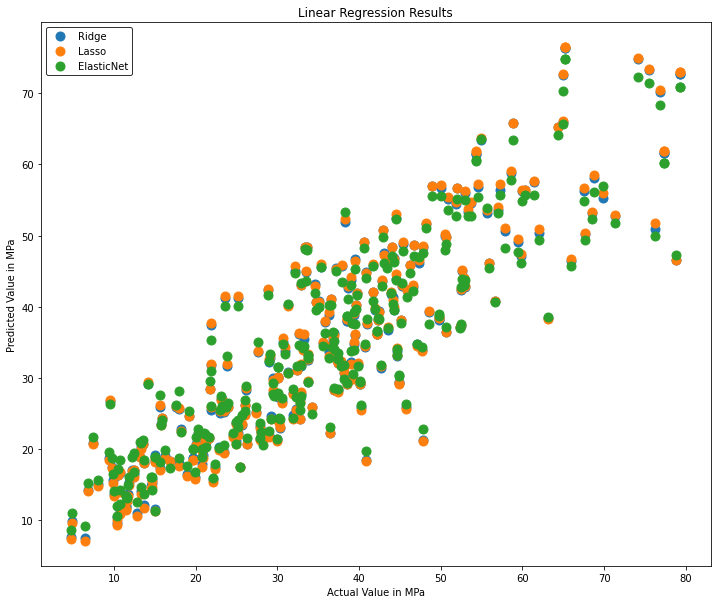
\includegraphics[width=\linewidth]{download.png}
  \caption{Linear Regression Results}
  \label{fig:boat1}
\end{figure}

It is natural to ask whether we can get lower errors if we apply the method of Stochastic Gradient Descent. Hereby, let us take the following extract from \href{https://scikit-learn.org/stable/modules/sgd.html}{scikit-learn $1.5.2$} user guide:

\medbreak

\begin{flushleft}
\texttt{"The class SGDRegressor implements a plain stochastic gradient descent learning routine which supports different loss functions and penalties to fit linear regression models. SGDRegressor is well suited for regression problems with a large number of training samples $(> 10.000)$, for other problems we recommend Ridge, Lasso, or ElasticNet."}
\end{flushleft}

\medbreak

In our analysis, our data has $1030$ samples in total. Therefore, it's not advisable to apply SGD.

\medbreak

Let us mention that by using statsmodels we obtain a slightly lower accuracy for our model. In any case, these results are very close to one another.

\medbreak

\begin{flushleft}
The value of MSE is given by $63.256$,\\ 
 and the value of R-Squared is given by $0.7699$.
\end{flushleft}

\medbreak

Finally, we highlight that the Elastic Net gives the best accuracy with $77.56\%$.
\section{Final Comments}\label{future}

The results regarding the regularization methods show that the margin of difference of error metric and scores of Ridge, Lasso, and Elastic Net are very tiny. By implementing the GridSearchCV, the gain of accuracy was of the order of $10^{-2}$, which again is insignificant. At the end of our analysis, we obtained that the Elastic Net gives the best accuracy. A natural question then arises, can we obtain better results? How can we proceed to that? Recall that in regularization methods we must remove the outliers, so our regression methods are not heavily penalized. So, is IQR our best option? Can we try other methods? If so, which ones? We believe that we should investigate this part in more detail in order to improve the accuracy. Surprisingly, statsmodels give a pretty descent accuracy. In the near future, we plan to explore more the tools from this library. 

\medbreak

Overall, we believe that our results are good, and acceptable if we take into account the features that we had to work with. A natural question that arises is, are there other important features to determine the strength of concrete? Common sense says that the answer is positive, so our next step is to explore these features. Let us mention that there are various types of concrete for different applications that are created by changing the proportions of the main ingredients. It would be challenging to get data from the different types of concrete, and analyse the results obtained by the techniques employed in this project. Of course, if we have more data samples (superior to $10.000$), we are tempted to apply the Stochastic Gradient Descent. Then, we would see whether the accuracy is greater. 
\end{document}